\newpage
\refstepcounter{section}
%Add Image
\vspace*{-40mm} %Make image have no top margin
\begin{tikzpicture}
\node[inner sep=0pt] (x) at (0,0)
    {\hspace{-87mm}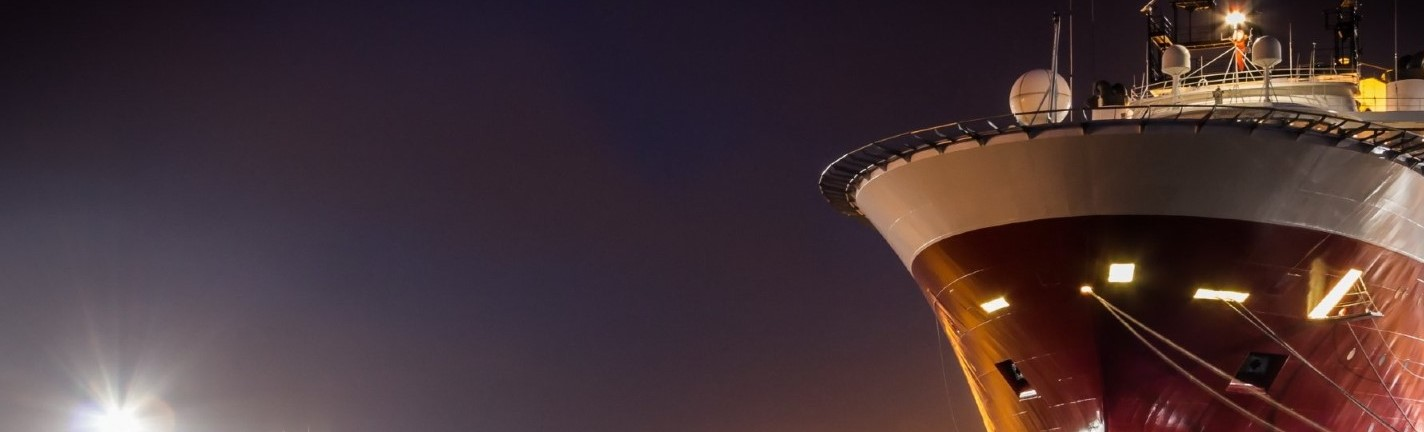
\includegraphics[width=\paperwidth]{sectionimage4.jpg}};
\node[text width=10in] (Z) at (0,-1) {\color{white}\headingfont\Large\bfseries\uppercase{\hspace{-0.7cm}\thesection\hspace{0.5cm}Safety}};
\end{tikzpicture}
%Modify TOC
\addcontentsline{toc}{section}{\protect\numberline{\thesection}Safety}
  \sectionmark{Safety}
\vspace{-5mm}

\begin{multicols}{2}
\subsection*{Emergency Protocols}
    \subsubsection*{During Construction}
        Following standard building site procedures, site workers would have safety gear on site (helmets, vests, boots etc), the site will be coned off from the public and caution will be exercised around existing pipelines, wires, drains and power lines. During the construction tunnels, the vibrations that are produced can trigger landslides or rock fall, possibly damaging the existing tunnel.
    \subsubsection*{Port}
        Internal programs and actions should be implemented to prevent any accidents to the best of the port’s abilities. This can include the identification of hazardous areas and ensuring there is sufficient signage. Additionally, sensible driving limits and pathways should be put in place to ensure the smooth proceedings within the port. Internal programs involve emergency contingencies; such as increased Fire Management Systems given the large oil tanks, lumber yard and fertilizer plant near by. Spill Management also needs to implemented, with increased training around managing an oil spill and boat inspections. Evacuation plans should be designed and designated with this in mind. Another program to consider would be Earthquake Preparation.
    \subsubsection*{Rail}
        During the design phases of the rail precaution should be taken to select appropriate safety factors to avoid derailing, technical failures and mechanical failures. In the case of fire prevention, flammable objects should be kept clear of the train lines. This is especially important in residential areas.The tunnel extension should take into account the ventilation so the construction workers have sufficient clean air and to improve visibility. The vibration caused by the construction of the tunnel can cause landslides/rockfall which can cause cracks in the existing rail line and pose a threat to the construction workers.
    \subsubsection*{Road}
        The areas affected by the road construction should be clearly marked with signs and outlined with reflective objects so drivers are aware of the construction and change of road. The speed limits around any roads that are under development should also be reduced. Construction should be conducted at night for areas that receive a lot of traffic to reduce the risk of collisions with both constructions workers and vehicles.

\subsection*{Accidents \& Fatalities}
    \subsubsection*{Port}
        As the hub of import and export for a majority of New Zealand’s freight, this is a 24/7, 365 days a year service. The number of workers needed to operate this port would need to be scaled to the work that goes into operation to prevent worker fatigue and any preventable accidents that result from this.
    \subsubsection*{Road}
        The use of more frequent passing lanes and double-laned development allows for safe  passing of the freight trucks that will be slower over the Gorge passes. Road shoulders should be frequent enough for vehicles to pull over into incase of emergency and the reflective safety barrier can be used during transitional road stages to prevent cars from going off the road. To prevent people from jaywalking, a sufficient amount of pedestrian crossings should be added in populated areas. The design of the road should make sure that the road is not susceptible to flooding by not passing through low points in valleys and elevating it above the surrounding ground level.
    \subsubsection*{Rail}
        Lines that pass through residential areas need to consider well designed rail crossings for both vehicles and pedestrians as well as fencing to prevent people from accessing the rail line. Upgrading the current Tauranga - Hamilton rail line would improve the safety factor and help prevent any derailing or engine failure. The concrete floor of the Kaimai track will need to be upgraded in order to accommodate the mass of 25 tonne trains. When constructed between 1969 and 1978, the tunnel floor was designed to take 18 tonne trains, so will need to be analysed in order to ensure structural integrity.

\end{multicols}
\clearpage